% !TEX root = ../Vorlage_DA.tex
%	########################################################
% 				Aufgabenstellung/Pflichtenheft
%	########################################################


%	--------------------------------------------------------
% 	Überschrift, Inhaltsverzeichnis
%	--------------------------------------------------------
\chapter{Grundlagen}

%	--------------------------------------------------------
% 	Was ist IoT?
%	--------------------------------------------------------
    \section{Was ist IoT?}\label{ref:IoT}
        IoT ist heutzutage nicht weg zu denken. Deswegen bedarf der Begriff an dieser Stelle einer Erklärung. 
        Das „Internet of Things“ (IoT oder auch zu Deutsch „Internet der Dinge“) verbindet Physisches und Virtuelles miteinander und publiziert dann im Endeffekt gesammelte Informationen. So sollen zum Beispiel immer kleiner werdende Computer, Menschen bei Tätigkeiten unterstützen. Diese werden sogar in Kleidung eingearbeitet, damit eingebaute Sensoren Daten sammeln können. Die Daten werden im Endschritt über das Internet publiziert, worüber man diese dann von überall auf der Welt einsehen kann. 
        
        \begin{figure}[H]
            \centering
            \includegraphics[width=0.5\textwidth]{./media/images/IoT.jpg}
            \caption{IoT Imagebild \cite{bib:betanews}}
            \label{fig:IoT}
        \end{figure}
        
        Eine weitere Veränderung, welche mit IoT kommt ist, dass veraltete Techniken von der Idee her komplett neu überarbeitet werden. Wie zum Beispiel bei einer normalen Klingel. Früher konnte sie nur eins: klingeln. Heute verfügen Klingeln über Bewegungssensoren, Kameras und Mikrofone, um einem über alles Bescheid zu geben was vor der Tür passiert.  
        
        IoT findet sich nicht nur im privaten Gebrauch. Ein Begriff, welcher große Gemeinsamkeiten aufweist wäre „Industrie 4.0“ (oder auch Industrial Internet). Beide Gebiete haben das Ziel, Geräte und Maschinen zu vernetzen.

\pagebreak


%	--------------------------------------------------------
% 	Energieeffiziente Systeme
%	--------------------------------------------------------
\section{Energieeffiziente Systeme}
Energy-Harvesting ist in dieser Diplomarbeit ebenfalls ein Thema, da eine Energie-autarke Stromversorgung für die Wetterstation nötig ist. Aber dann stellt sich die Frage: Was ist Energy-Harvesting eigentlich?

\begin{figure}[H]
    \centering
    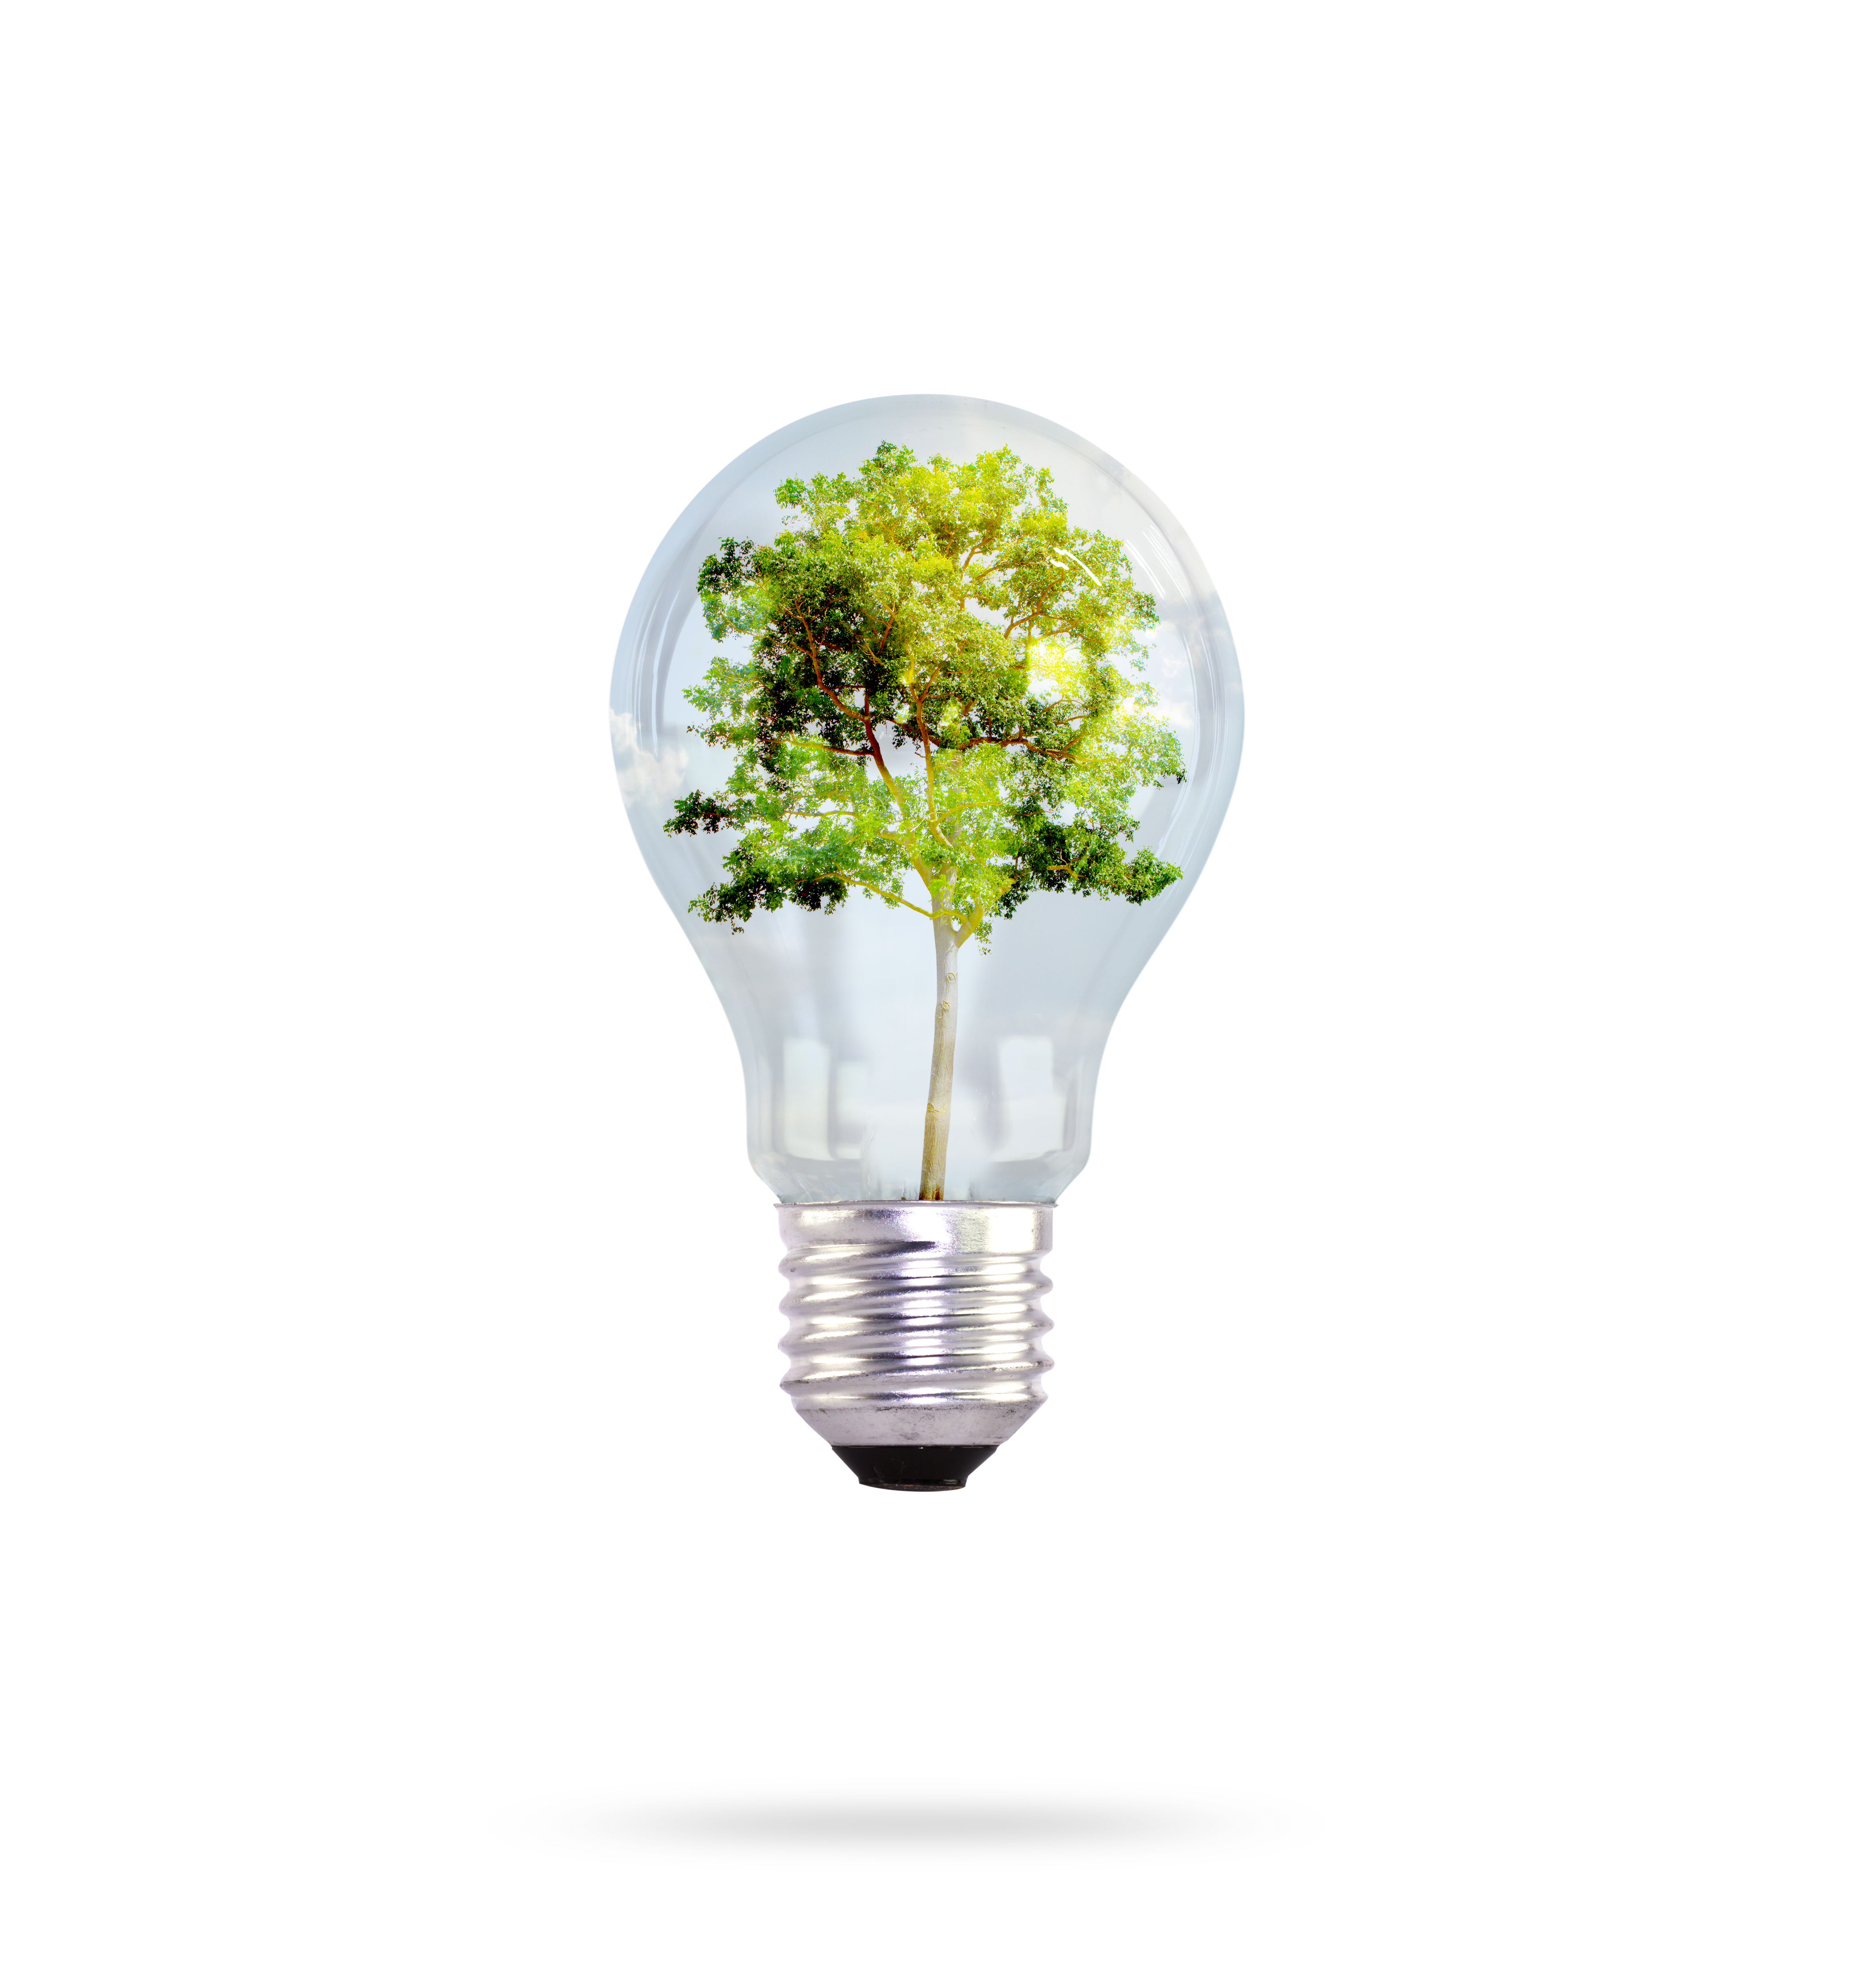
\includegraphics[width=0.7\textwidth]{./media/images/greenenergy.jpg}
    \caption{Green Energy Imagebild \cite{bib:genergy}}
    \label{fig:genergy}
\end{figure}

Beim Energy-Harvesting geht es grundsätzlich darum, die verlorene Energie einer Funktionalität zumindest teilweise wiederzuverwerten. Es ist ja zurzeit so, dass wir Energiequellen nicht vollkommen effektiv nutzen. Man nehme zum Beispiel Kohlekraftwerke: Diese haben heutzutage einen Wirkungsgrad von 40\% \cite{bib:kohle}. 

Energy-Harvesting ist im speziellen jedoch für kleinere Projekte mit niedrigem Stromverbrauch gedacht. Wie zum Beispiel für eine kleine Wetterstation. Andere Anwendungsbeispiele wären zum Beispiel Uhren, welche durch Erschütterung ihre Energie beziehen oder Sensoren, welche dank Wärmeeinstrahlung funktionieren.
